\documentclass{article}

\usepackage{comment}
\usepackage{graphicx}
\graphicspath{ {./images/} }
\usepackage{float}

\renewcommand\thesection{\Roman{section}.}


\title{HERE Technologies Research Proposal}


\begin{document}
	\pagenumbering{gobble}
	\maketitle
	\newpage
	\pagenumbering{arabic}
	
	\begin{abstract}
		Mapping the surrounding environment is of utmost importance for path planning and obstacle avoidance of Autonomous Vehicles. In this report we would like to propose an innovative system that would create a dense 3D geometric map of complex urban environment with additional Geo-spatial information to reduce the computational complexity of Autonomous Driving. Our system would also be able to classify static and dynamic obstacles, identify and map static land marks and remove dynamic obstacles from the map.
		
	\end{abstract}
	
	\section{Introduction}
		\paragraph{}
		Autonomous vehicles have the potential to revolutionize the transportation industry by drastically improving safety and efficiency of transportation. In order to navigate through complex environments the vehicles rely on wide array of sensors like Light Detection And Ranging (LiDAR), Camera, Inertial Measurement Unit (IMU), Global Navigation Satellite System (GNSS). The level of autonomy in Autonomous Driving Systems is determined by its ability to perceive and navigate in complex environments. Simultaneous Localization And Mapping (SLAM) has been an active area of research in Robotics
		\cite{durrant-whyte_simultaneous_nodate}
		\cite{bailey_simultaneous_2006}.
		To accomplish this task the system needs to sense and generate an accurate map of the environment using different SLAM techniques, find its location in the map using Monte Carlo Localization
		\cite{thrun_robust_2001}
		or Kalman filter based localizations 
		and navigate to the destination. Several approaches have been proposed 
		\cite{durrant-whyte_simultaneous_nodate}
		\cite{thrun_graph_2006},
		however the most successful one
		\cite{levinson_map-based_2007}
		was developed by Stanford Artificial Intelligence Lab. 
		
		Most of the related work conducted has been focused on very specific and constrained environments, however to achieve a fully autonomous system, the challenge of mapping large-scale environments needs to be tackled. The objective of this project is to develop a system that can not only generate a three dimensional large-scale map but also add more detailed information to the map data.
	
	\begin{comment}
	Autonomous vehicles require more information that the standard 2D map provides. It needs to understand when and where to look for traffic signals, speed limits. Even to perform a simple task like taking a turn, the autonomous vehicle requires information like where the turn only lane starts which isn't provided in standard maps. Hence we need maps that have more data that simple latitude and longitudinal data.
	Perception and navigation in complex environment requires a well defined map of the environment. LiDAR is usually used to generate a map of the environment using the 3D point cloud data. Camera's do not directly provide a depth perception but can be extremely efficient in image classification and obstacle detection.
	
	\underline{\textit{How Self driving requires more data than just the data provided by GNSS}}
	\end{comment}
	
	\section{Related Work}
		\paragraph{}
		Different Mapping Techniques that have been deployed for generating map data can be broadly classified into 
		LiDAR Mapping
		\cite{levinson_robust_2010},
		Visual Mapping
		\cite{liu_towards_nodate}
		\cite{Krombach_Droeschel_Behnke_2017}
		and Sensor Fusion based Mapping
		\cite{silva_fusion_nodate}. 
		LiDAR based mapping is usually preferred as it generates accurate point clouds data which provide a depth perception of the image. This depth information is extremely useful in navigation. Visual mapping is primarily based on camera data. Unlike LiDARs, Cameras require ambient lighting and cannot provide depth information by default. However, cameras provide better scene segmentation and understanding
		\cite{heng_project_2018}.
		We can also use multi camera system
		\cite{geiger_stereoscan:_2011}
		to gain depth perception along with different wide field of view lenses or fisheye lenses
		\cite{cui_real-time_2018}
		to gain more information.
		The sensor fusion based approach tries to combine the data from all the sensors and generates a map that has a depth perception of LiDAR as well as better scene segmentation of Camera. Other sensors commonly used are RADAR for navigation and obstacle detection, IMU and GNSS for better localization.
		Figure 1 lists all the advantages and drawbacks of different sensors and provides a graphical explanation of how sensor fusion helps in overcoming individual sensor shortcomings.
	
			\begin{figure}[H]
				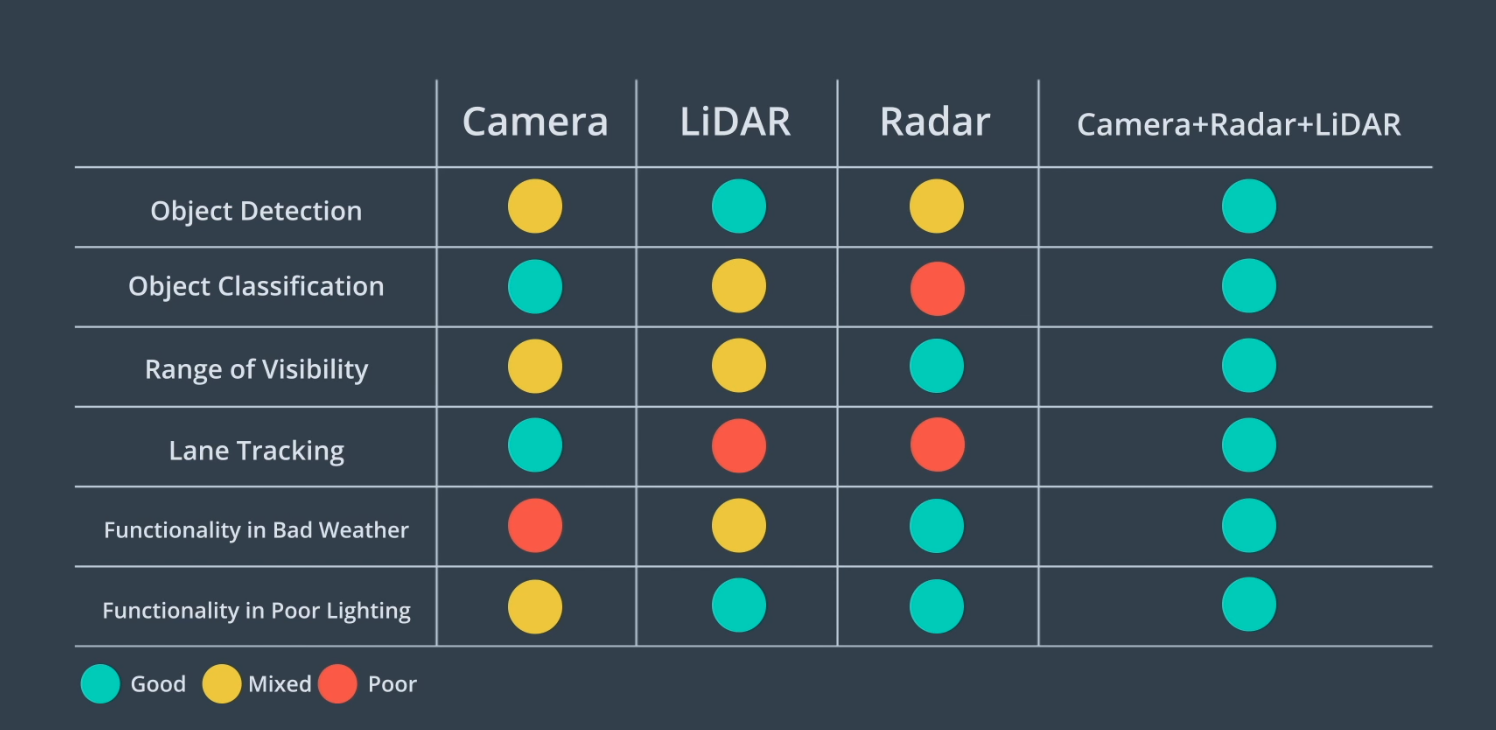
\includegraphics[width=\textwidth]{Sensor_Comparison}
				\caption{Sensor Comparison
				\cite{noauthor_self-driving_nodate}}
			\end{figure}
	
		
		The data collected from all these sensors is then processed and map is generated. 
		Different map generation methods for unknown map environments are based on probabilistic frameworks. In the case of autonomous vehicles the real-time map generation is very computationally intensive, needs very heavy optimization. The online probabilistic algorithms are based on Markov assumption to estimate the current pose and generate map agnostic of the previous data collected about the same environment.
		Markov assumption states that past information is irrelevant if pose and map is known.
		This assumption helps in reducing the computational complexity and is very useful in small-scale environments
		\cite{mutz_large-scale_2016}.
		The most commonly used online algorithms are Unscented Kalman Filter
		\cite{thrun_probabilistic_2005},
		FastSLAM
		\cite{montemerlo_fastslam:_2002}
		and FastSLAM 2.0
		\cite{montemerlo_fastslam:_2007}.
		The offline set of probabilistic algorithms integrate previous and present data to estimate previous set of poses visited by the vehicle and generate the map based on it. GraphSLAm is one of the most successful implementations of offline Full-SLAM (offline algorithms that estimate the entirety of previous poses)
		\cite{thrun_graph_2006}.
		
	\section{Proposed Mapping Technique}
		\paragraph{}
		We propose a system which builds on previously mentioned work and improves on it by focusing on two major aspects:
			\begin{itemize}
				\item Reusing Prior Maps
				\item Adding more information to Existing Map Data
			\end{itemize}
	
			\begin{figure}[H]
			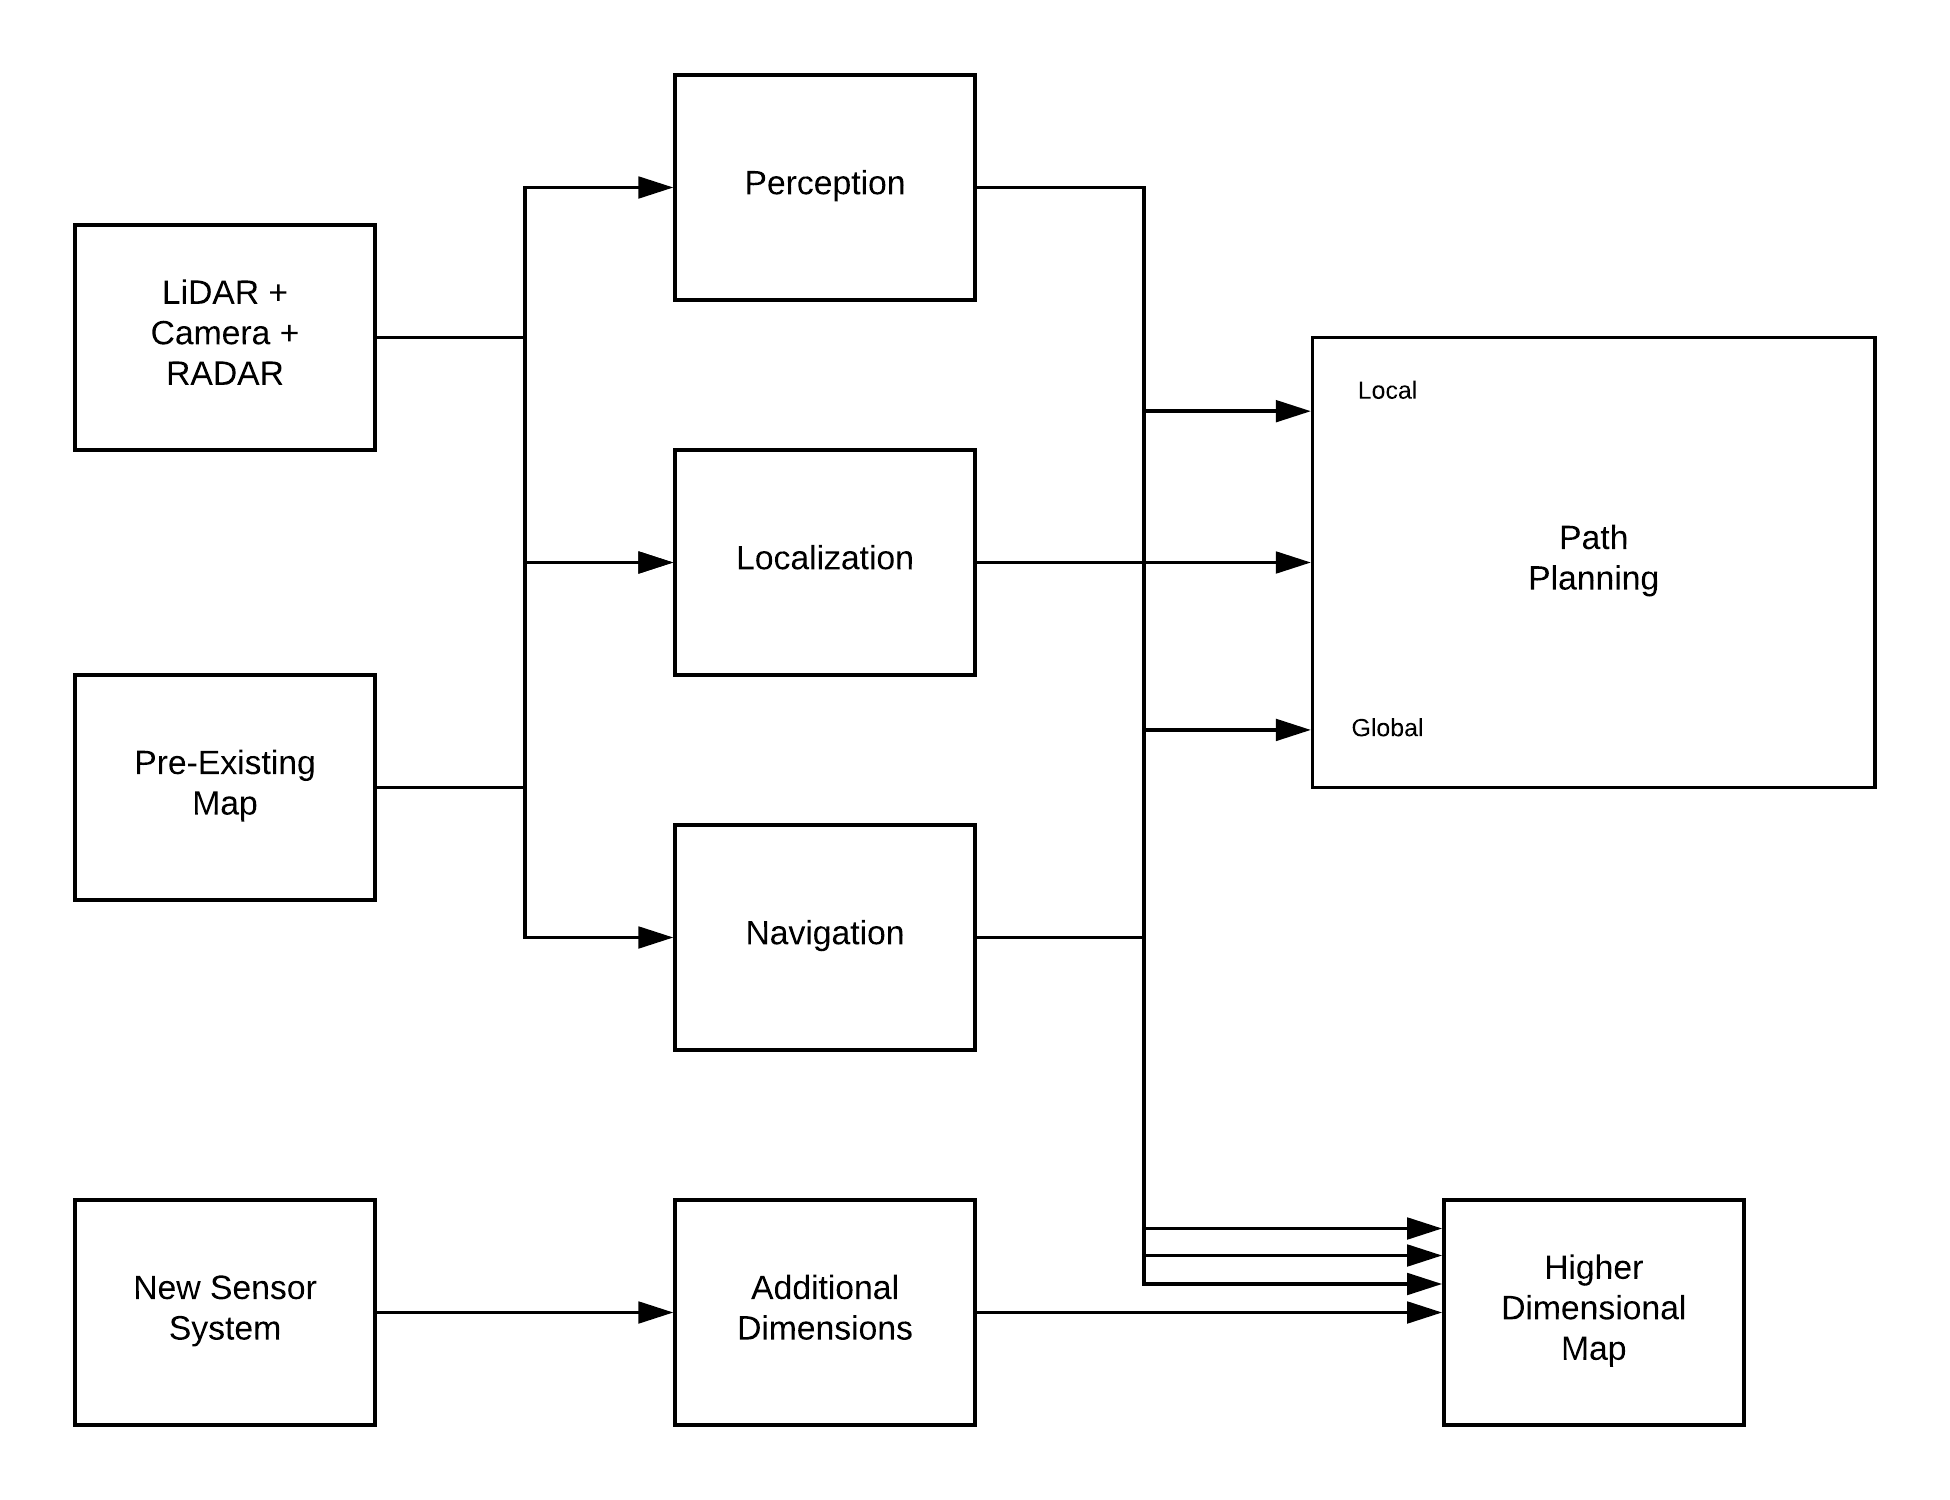
\includegraphics[width=\textwidth]{HERE_Proposed_System}
			\caption{Proposed System}
			\end{figure}
		
		The proposed system would focus on classification of dynamic and static obstacles in the path using visual motion estimation. This approach tries to determine motion by performing an optimized frame-by-frame comparison
		\cite{Krombach_Droeschel_Behnke_2017}.
		We can further optimize this approach by validating it with a LiDAR based iterative closest point algorithm. We can use this identification of dynamic objects
		\cite{kiran_real-time_2018}
		to mask them in our mapping algorithm to further improve the quality of information in our map data.
		
		
	\section{Conclusion}
		\paragraph{}
		We propose a novel system which develops a feedback loop with the system, thereby improving the quality of map data with every iteration. This increased information in map data would reduce the computational complexity of the already complex task of autonomous driving.
	
	
\newpage
\bibliographystyle{IEEEtran}
\bibliography{ResearchProposal}

\end{document}
